% Chapter 18 - Proteins.tex
% Copyright (c) 2014 - 2016, zhiayang@gmail.com
% Licensed under the Apache License Version 2.0.

\pagebreak
\hypertarget{ChapterProteins}{}
\part{Proteins}


	\section{Protein Structure}

		Proteins are essentially polypeptide chains with a relative molecular mass that is greater than 5000. Proteins are, as one might
		guess, essential to the functioning of life, with structural, transportational, and catalytic functions.

		The structure of proteins can be described in a roughly hierarchical fashion with 4 tiers.

		\subsection{Primary Structure}

			The primary structure of a protein is the simplest to describe; it is simply the order and composition of the polypeptide chain
			that makes up the protein.

		% end subsection


		\subsection{Secondary Structure}

			The secondary structure of a protein is the \itl{regular arrangement} of \itl{sections} of the primary polypeptide chain into either
			α-helices or β-pleated sheets. Note that there are still sections of the polypeptide chain that simply exist as
			strands, and are not regularly arranged.

			Both α-helices and β-pleated sheets are held in place by hydrogen bonds between the atoms in the \itl{peptide bond},
			and nowhere else. Since these bonds occur regularly along the chain, they naturally facilitate the formation of these regular
			arrangements.

			\diagram[0.80]{
				\chemfig{C(=[:180]!\molO)(-[:300])(-[:60]\chemabove{\color{RoyalBlue}N}{\hspace{1mm}\smdeltam}(-[:0]\chemabove{H}{\hspace{1mm}\smdeltap}-[:0,2.0,,,dashed]\dotlewis{\color{Red}O}{180}=[:0]C(-[:60])(-[:300]!\molN(-[:240]H)(-[:0])))(-[:120]))}
			}

			Of course, there are other secondary structures other than α-helices and β-sheets, such as the π-helix, reverse helices, etc.
			However, these two are the most common secondary structure in proteins.


			\pagebreak
			\subsubsection{\chemalpha-helices}

				α-helices form when the polypeptide chain twists into a clockwise spiral; due to the positions of the
				hydrogen bond-forming peptide linkages, each turn of the helix has \itl{3.6} residues. The R groups face outwards, allowing for
				residues with bulky R groups to form helices as well.

				All the \ch{C=O} bonds point in one direction, while all the \ch{N-H} bonds point in the opposite direction; both run parallel
				to the spine of the helix.

				\imgdiagram{100mm}{../figures/organic/ch18/alpha_helix.png}

			% end subsubsection


			\subsubsection{\chembeta-pleated sheets}

				β-sheets are formed when two sections of a polypeptide chain find themselves parallel to each other, allowing the peptide bond
				atoms to face their counterpart on the other chain to form hydrogen bonds.

				The carbonyl and amide groups are oriented \itl{along} the plane of the sheet, while the R-groups of each residue face either
				upwards or downwards from the sheet.

				\begin{figure}
				\begin{center}
					\begin{subfigure}{.5\textwidth}
						\centering
						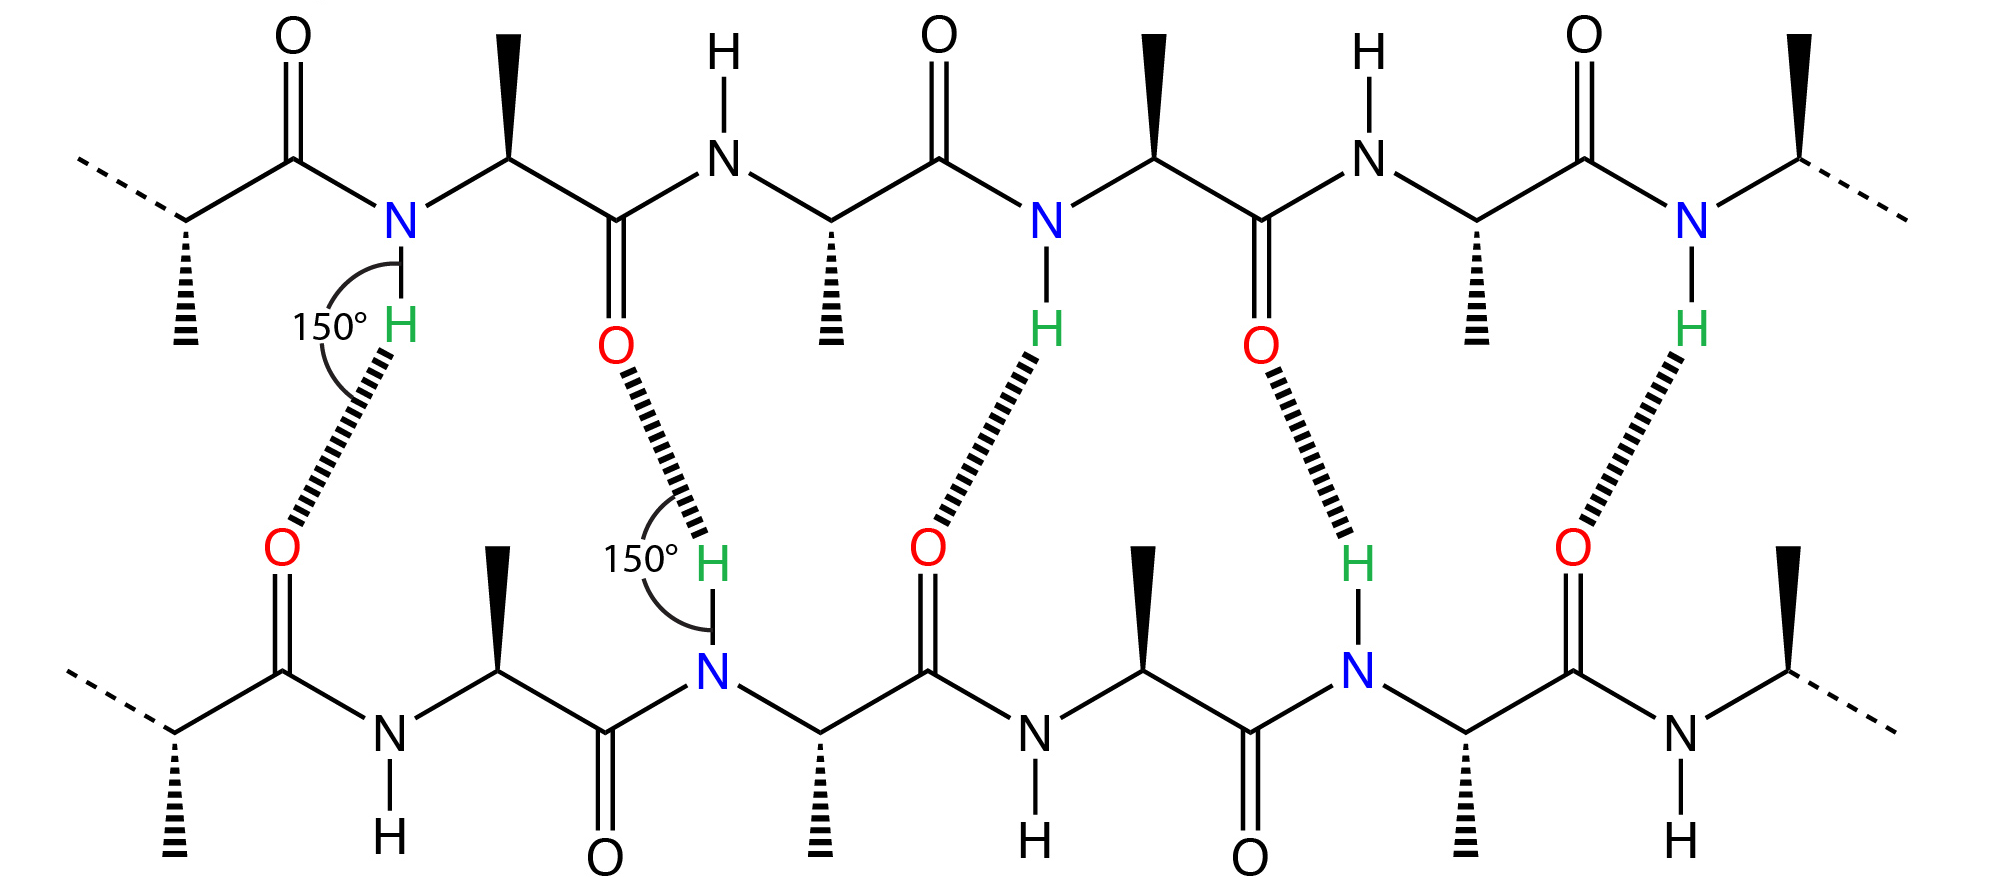
\includegraphics[width=80mm]{../figures/organic/ch18/parallel_beta_sheet.png}
						\caption*{Parallel β-sheet}
					\end{subfigure}%
					\begin{subfigure}{.5\textwidth}
						\centering
						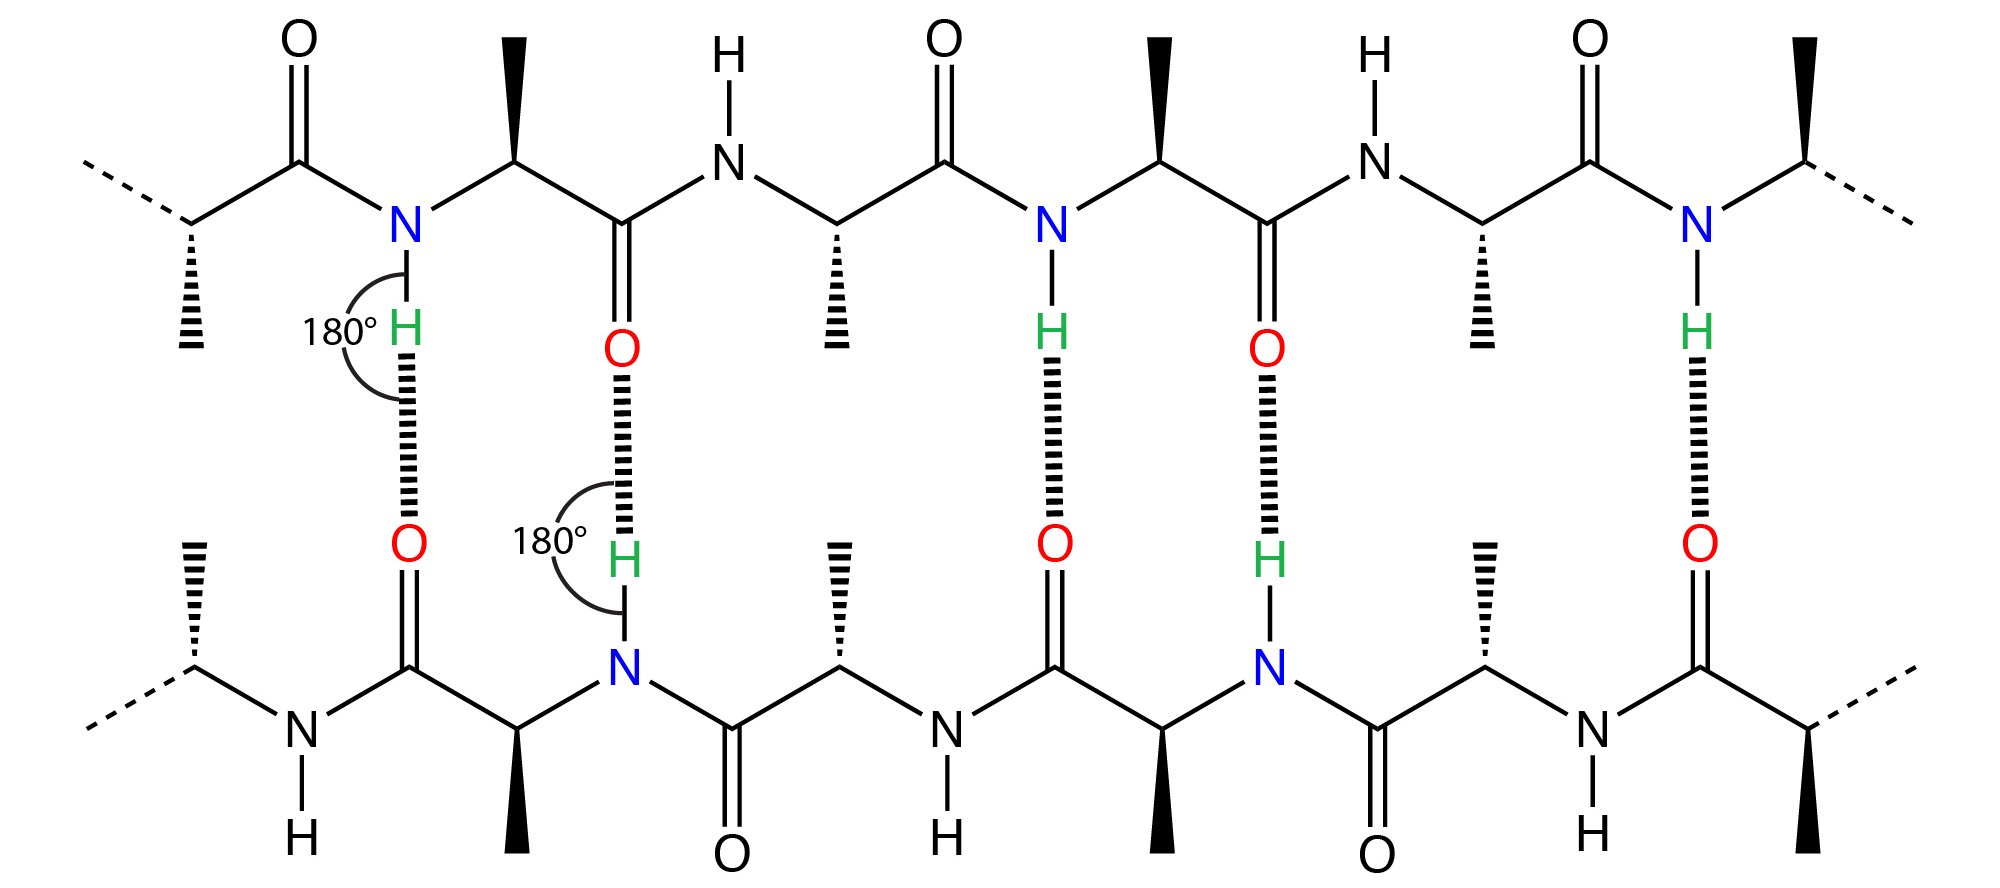
\includegraphics[width=80mm]{../figures/organic/ch18/antiparallel_beta_sheet.png}
						\caption*{Antiparallel β-sheet}
					\end{subfigure}
				\end{center}
				\end{figure}

				There are \itl{parallel} and \itl{antiparallel} varieties of β-sheets, where the two strands either run in the same direction,
				or in opposite directions.

			% end subsubsection

		% end subsection


		\subsection{Tertiary Structure}

			The tertiary structure of a protein is mainly concerned with the bonding and interactions between the \itl{R-groups} of the
			amino acid residues in the polypeptide chain.

			The overall 3-dimensional arrangement of the protein is determined mainly by the kinds of tertiary interactions that are
			present; there are 4 main kinds of interactions that allow the tertiary structure to take shape.

			\subsubsection{Ionic Interactions}

				At certain \pH{} levels, carboxylic acid and amine groups in side chains can be ionised, and thus they can form ionic
				interactions between them.

				For example, at some \pH{} level, the \ch{CO2-} group in one side chain can form ionic interactions with the \ch{NH3+} group
				in a neighbouring side chain.

			% end subsubsection


			\subsubsection{Hydrogen Bonds}

				Hydrogen bonding between side chains is distinct from the hydrogen bonding that maintains the secondary structure of the protein.
				These hydrogen bonds can form between any polar group in the side chain, for example alcohols, phenols, amides, amines, etc.

			% end subsubsection


			\subsubsection{Id-id Interactions}

				These \idid{} interactions are present with any alkyl group in the side chain, and of course become
				stronger with larger R groups; benzene rings are particularly good at these.

			% end subsection


			\subsubsection{Disulphide Bridges}

				When two thiol \ch{S-H} groups are in close proximity, the sulphur atoms can form a strong covalent bond (\ch{S-S}) between them,
				forming a disulphide bridge (hence the name).

			% end subsubsection

		% end subsection


		\subsection{Quaternary Structure}

			The quaternary structure of a protein is relevant when a protein has \itl{more than one} polypeptide chain. Each polypeptide chain
			can have its own primary, secondary, and tertiary structures, and are linked together via the quaternary interactions to form the
			overall protein.

			Examples of these include insulin, which consists of 2 chains, or haemoglobin, consisting of 4 chains.

		% end subsection

	% end section



	\section{Enzymes}

		Enzymes are biological catalysts that are highly specific, due to the nature of their mechanism. The active sites of an enzyme rely on
		tertiary interactions to bond to the substrate that is being catalysed, so only specific molecules can fit into the active site.

		When an enzyme is denatured, its tertiary structure is disrupted, thus changing the structure of its active site. This prevents it
		from binding to the molecule that it is supposed to, and the enzyme loses its function.

	% end section



	\section{Denaturation of Proteins}

		There are many ways that proteins can be denatured, all involving the disruption or destruction of the secondary, tertiary and quaternary
		structures of the proteins. Note that the primary structure, ie. the peptide linkages, remain intact in a denatured protein.

		Since proteins rely on said structures to perform their job (like enzymes), denatured proteins are effectively useless, and these
		changes are typically irreversible. Eggs do not un-fry when you put them back in the fridge, for instance.


		\subsection{Heat}

			The most basic form of denaturation simply involves heating the protein, thus providing energy to break the secondary and tertiary
			interactions and hence destroying its structure.

			Since the regular structures are destroyed, a side effect of heat-induced denaturation is that the protein exists mostly as a mess
			of unfolded chains; this typically results in \itl{coagulation}, due to the entanglement of said chains.

			Examples of this kind of denaturation are plenty, eggs and meat both contain plenty of proteins that are denatured with heat,
			turning firm.

		% end subsection


		\subsection{\MpH{} Changes}

			\pH{} changes primarily serve to either protonate or deprotonate the acid and amine groups in the side-chains of the residues,
			disrupting both hydrogen bonding and ionic interactions between said side-chains.

			At low \pH{} levels, groups are protonated, forming \ch{CO2H} and \ch{NH3+} --- the acid groups no longer form ionic interactions,
			while the amine groups no longer form hydrogen bonds (since the N atom becomes positively charged).

			At high \pH{} levels, groups are deprotonated, having the opposite effect; \ch{CO2-} can no longer form hydrogen bonds, and
			\ch{NH2} can no longer form ionic interactions.

		% end subsection


		\subsection{Metal Ions}

			Metal cations tend to form ionic interactions preferentially with \ch{CO2-} groups in the side chain, thus disrupting the tertiary
			and quaternary structures of proteins that they bind to.

			Separately, some heavy metal ions like silver, mercury and lead will bind to the sulphur atom, disabling the disulphide bridges in
			those areas.

		% end subsection


		\subsection{Mechanical Agitation}

			Some of the weak interactions at the tertiary or quaternary level can be disrupted simply by the act of shaking or stirring,
			which leads to the uncoiling of the structure. Eggs exhibit this behaviour, as their texture and composition change significantly
			when whipped.

		% end subsection


		\subsection{Solubility-enhancing Substances}

			Certain substances like detergents can bind to typically insoluble alkyl side-chains, disrupting the original id-id interactions that
			were in place.

		% end subsection

	% end section



	\section{Hydrolysis of Proteins}

		Since proteins are essentially long polypeptide chains, they too can be hydrolysed, requiring several hours of heat in an acidic or
		alkaline solution. Partial hydrolysis will yield a mixture of different products in various stages of breakdown.

		Note that hydrolysis is distinct from denaturation; the latter involves destroying the secondary, tertiary and quaternary structures
		of the protein, while hydrolysis involves breaking the \itl{peptide linkages} themselves, destroying the primary structure.

	% end section


% end part
